\subsection{降温法}
降温法是从溶液中培养晶体的一种最常用的方法。这种方法适用于溶解度和温度系数都较大的物质,并需要一定的温度区间。这一温度区间也是有限制的:温度上限由于蒸发量大而不宜过高,当温度下限太低时,对晶体生长也不利。一般来说,比较合适的起始温度是50---60℃,降温区间以15---20℃为宜。

降温法的基本原理是利用物质较大的正溶解度温度系数,在晶体生长过程中逐渐降低温度,使析出的物质不断在晶体上生长。用这种方法生长的物质的溶解度温度系数最好不低于1.5g/1000g$\text{溶液}\cdot$℃,表3.7列出符合此要求的一些物质的数据。

\begin{table}[h]
\centering
\caption{40℃时,一些物质的溶解度及其温度系数}
\begin{tabular}{c|c|c}\toprule
物质 & \tabincell{c}{溶解度\\(g/1000g溶液)} & \tabincell{c}{溶解度温度系数\\g/1000g$\text{溶液}\cdot$℃}\\\hline
明矾\quad$\rm K_2SO_4\cdot Al_2(SO_4)_3\cdot 24H_2O$ & 240 & $+9.0$\\
ADP\quad$\rm NH_4H_2PO_4$ & 360 & $+4.9$\\
TGS\quad$\rm (NH_2CH_2COOH)_3\cdot H_2SO_4$ & 300 & $+4.6$\\
KDP\quad$\rm KH_2PO_4$ & 250 & $+3.5$\\
EGT\quad$\rm ???$ & 598 & $+2.1$\\
\bottomrule
\end{tabular}
\end{table}

降温法生长晶体的几种装置,如图3.18、图3.19和图3.20所示。

在降温法生长晶体的整个过程中,必须严格控制温度,并按一定程序降温。研究表明,微小的温度波动就足以在生长的晶体中造成某些不均匀区域。为提高晶体生长的完整性,要求控温精度尽可能高(目前已达±0.001℃),此外还需造成适合晶体生长的其他条件。

\begin{figure}[h]
 \centering
 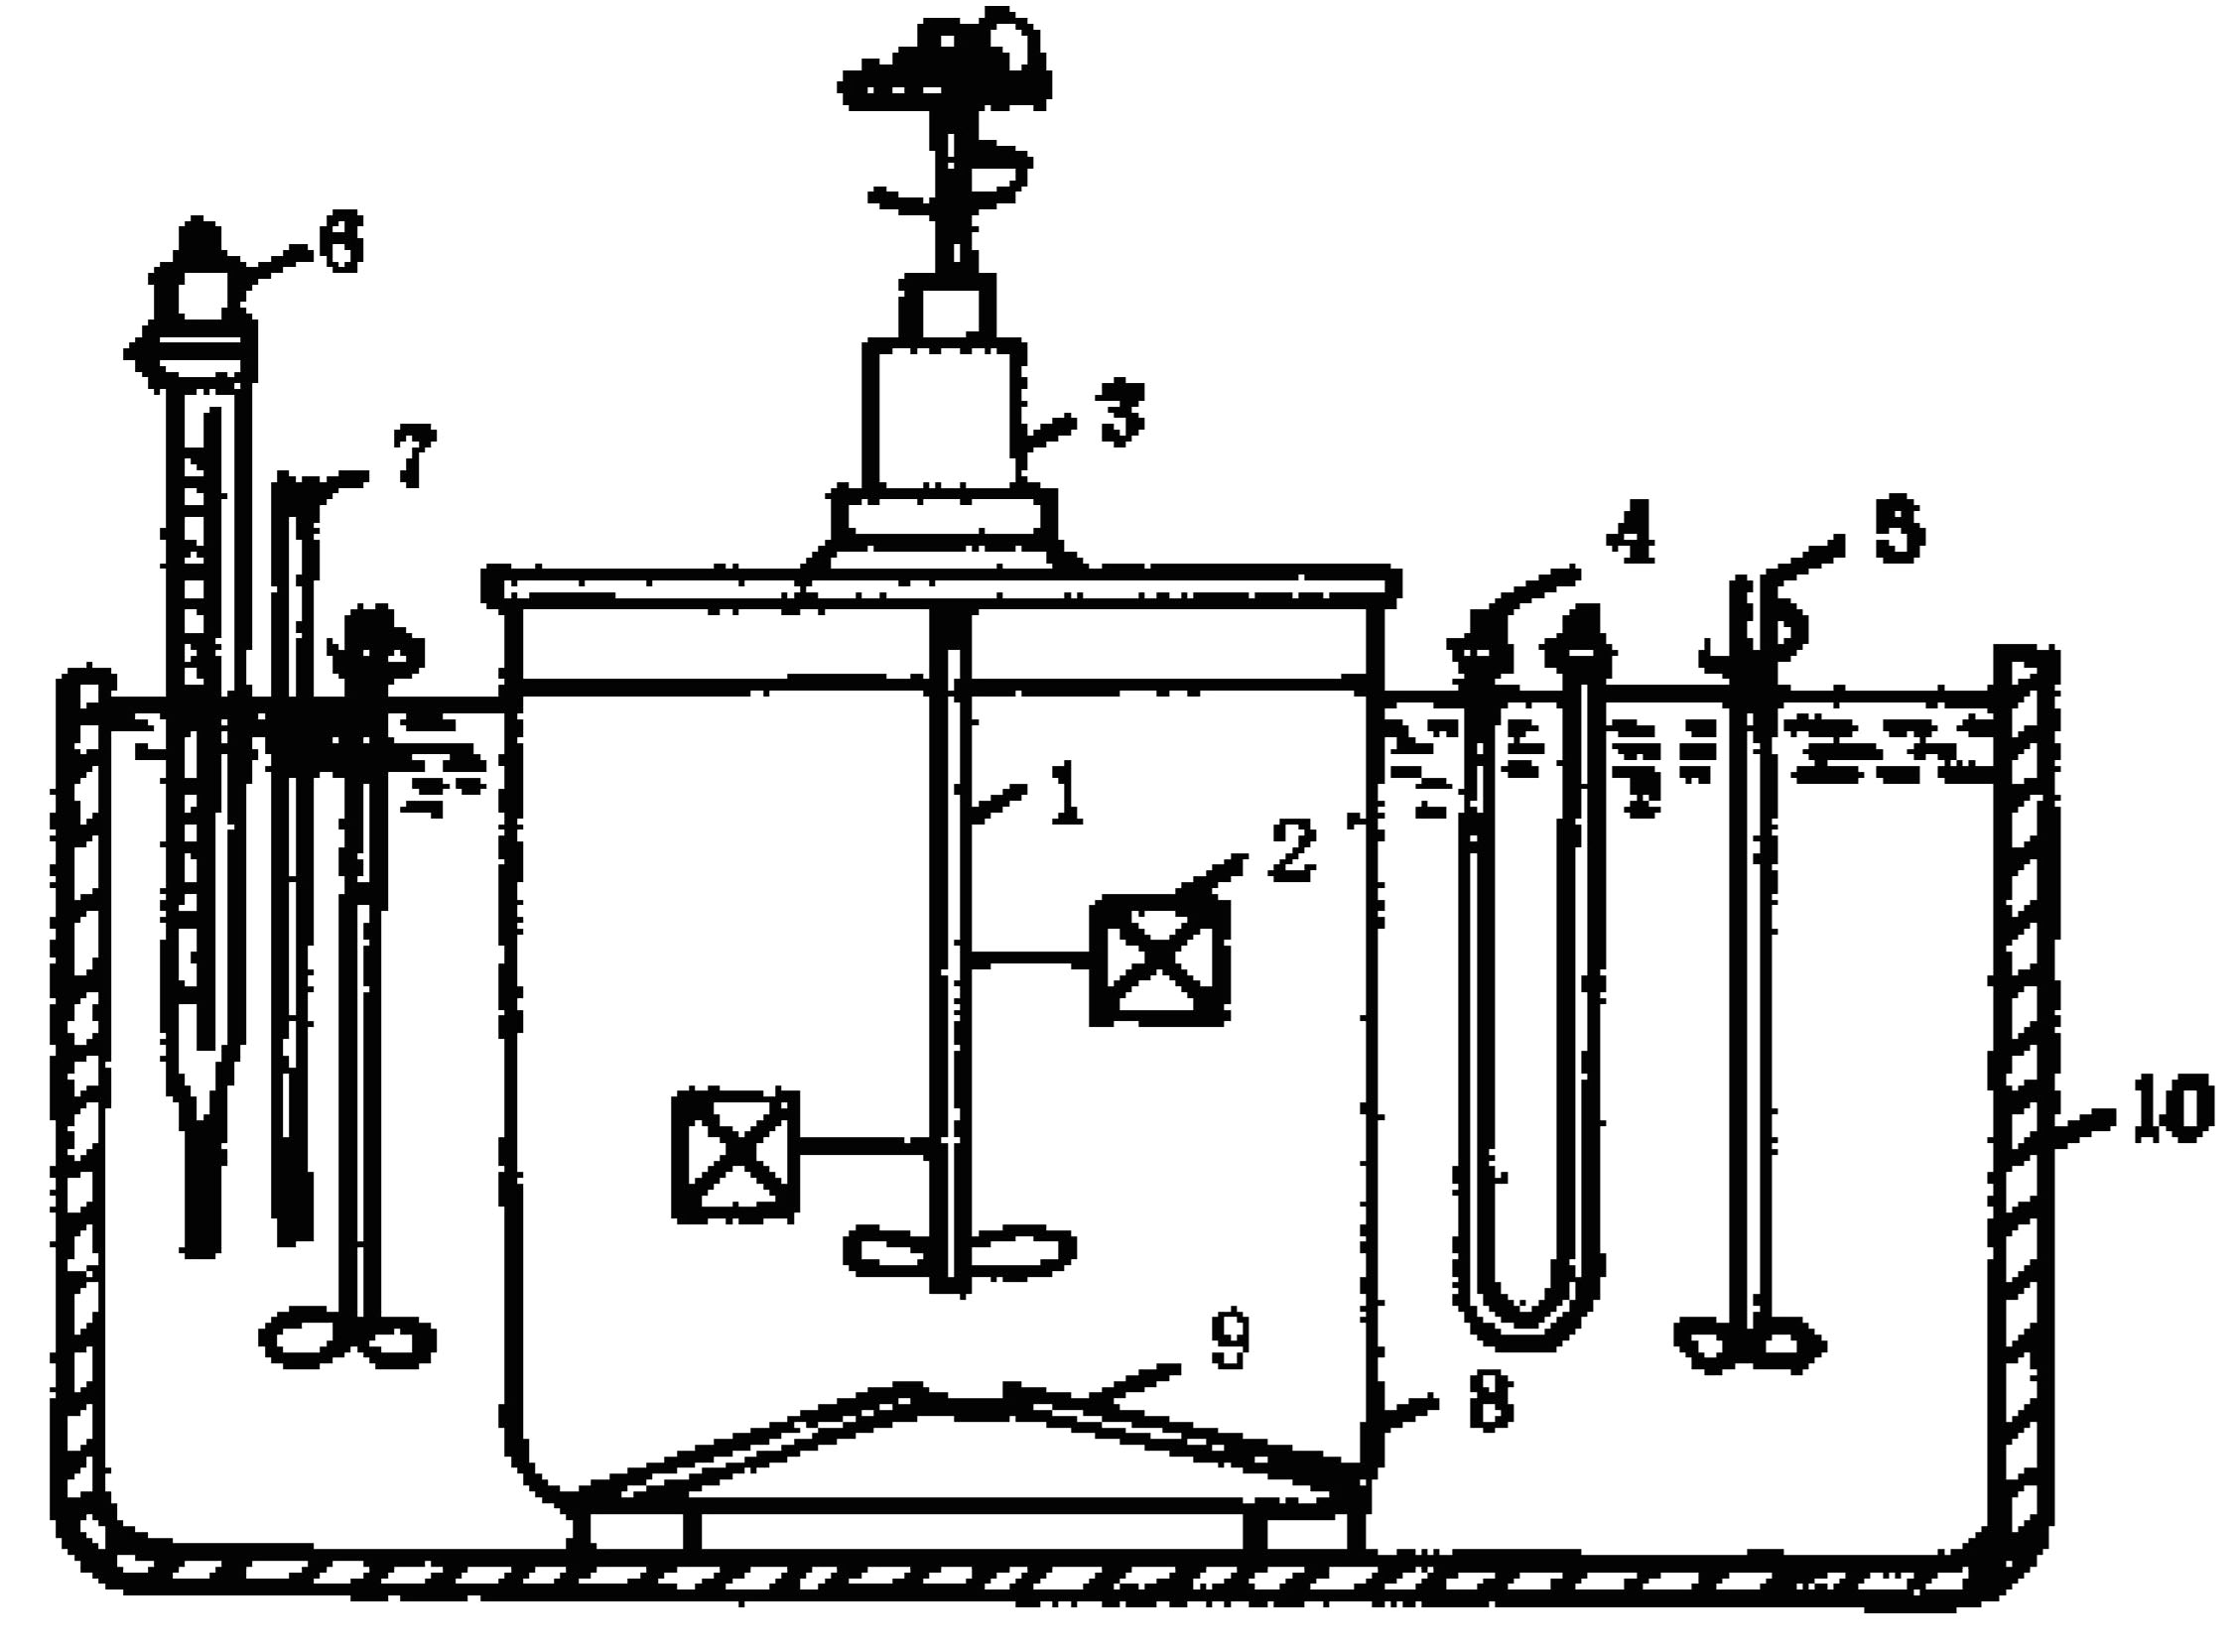
\includegraphics[width=0.5\textwidth]{fig/cp03/img3.18.jpg}
 \caption{水浴育晶装置。图中:}
 1为掣晶杆;2为晶体;3为转动密封装置;4为浸没式加热器; \\
 5为搅拌器;6为控制器(接触温度计);7为温度计;8为育晶器;\\
 9为有孔隔板;10为水槽。
\end{figure}

在利用降温法来生长晶体的过程中可不用再补充溶液或溶质。因此,整个育晶器在生长过程中必须严格密封,以防溶剂蒸发和外界的污染。例如从重水溶液中生长晶体时,如果密封不好,溶液中的D$_2$O就会同大气中的H$_2$O汽发生同位素交换而使溶液氘化程度下降。为增加温度的稳定性,育晶器的容量必须要大些(大型育晶器有几十升至上千升),加热保温方式有水浴槽或内部加热、外壳加保温套等。育晶器顶部经常有保持冷凝水回流,底部有电炉加热为好,使得溶液表面和底部都有不饱和层保护,避免自发晶核形成。

育晶器内的控温精度除了与育晶装置的结构有关外,很大程度上取决于控温装置,继电器开关式控温一般可以满足水溶液晶体生长的要求,温度波动可以控制在±0.05℃以下,用PID控温方式,特别是使用可编程温度控制器控温,实现控温精度至±0.005℃并不困难,这对培养高完整性单晶十分有利。

\begin{figure}[htb]
 \centering
 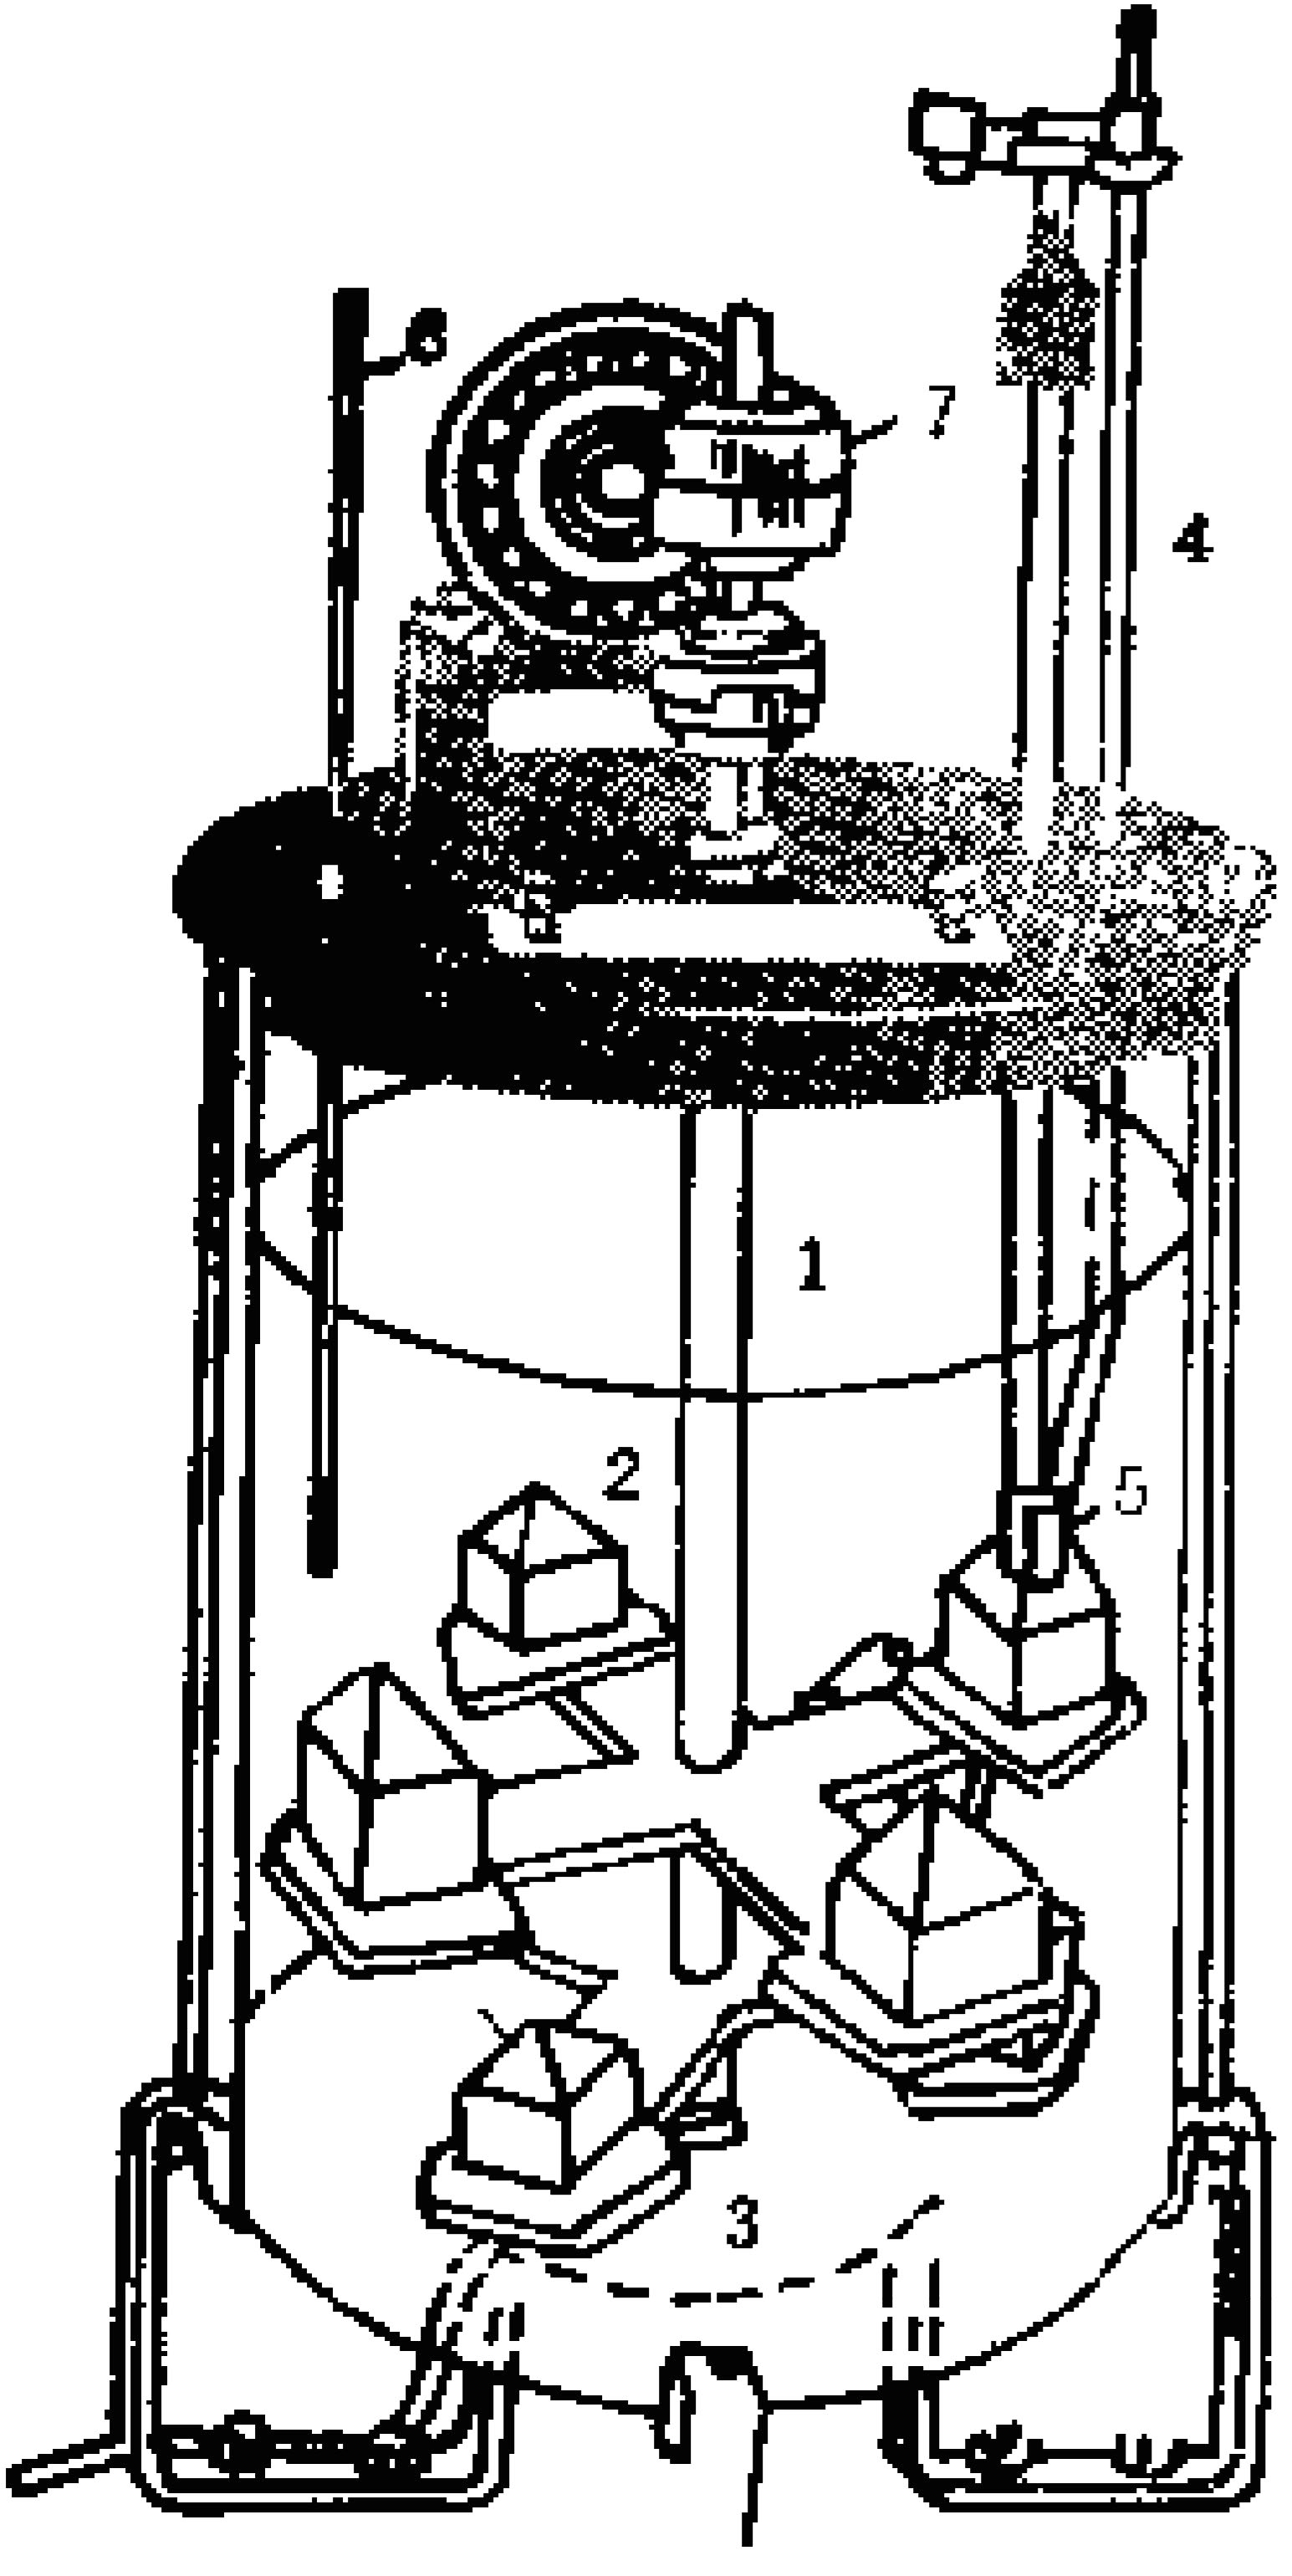
\includegraphics[width=0.3\textwidth]{fig/cp03/img3.19.jpg}
 \caption{直接加热的转动育晶器。}
 图中:1为掣晶板;2为晶体;3为底部主加热器;4为控制器; 5为辅助小灯泡加热器;6为温度计;7为可逆转动装置(30r/min)。
\end{figure}

\begin{figure}[htb]
 \centering
 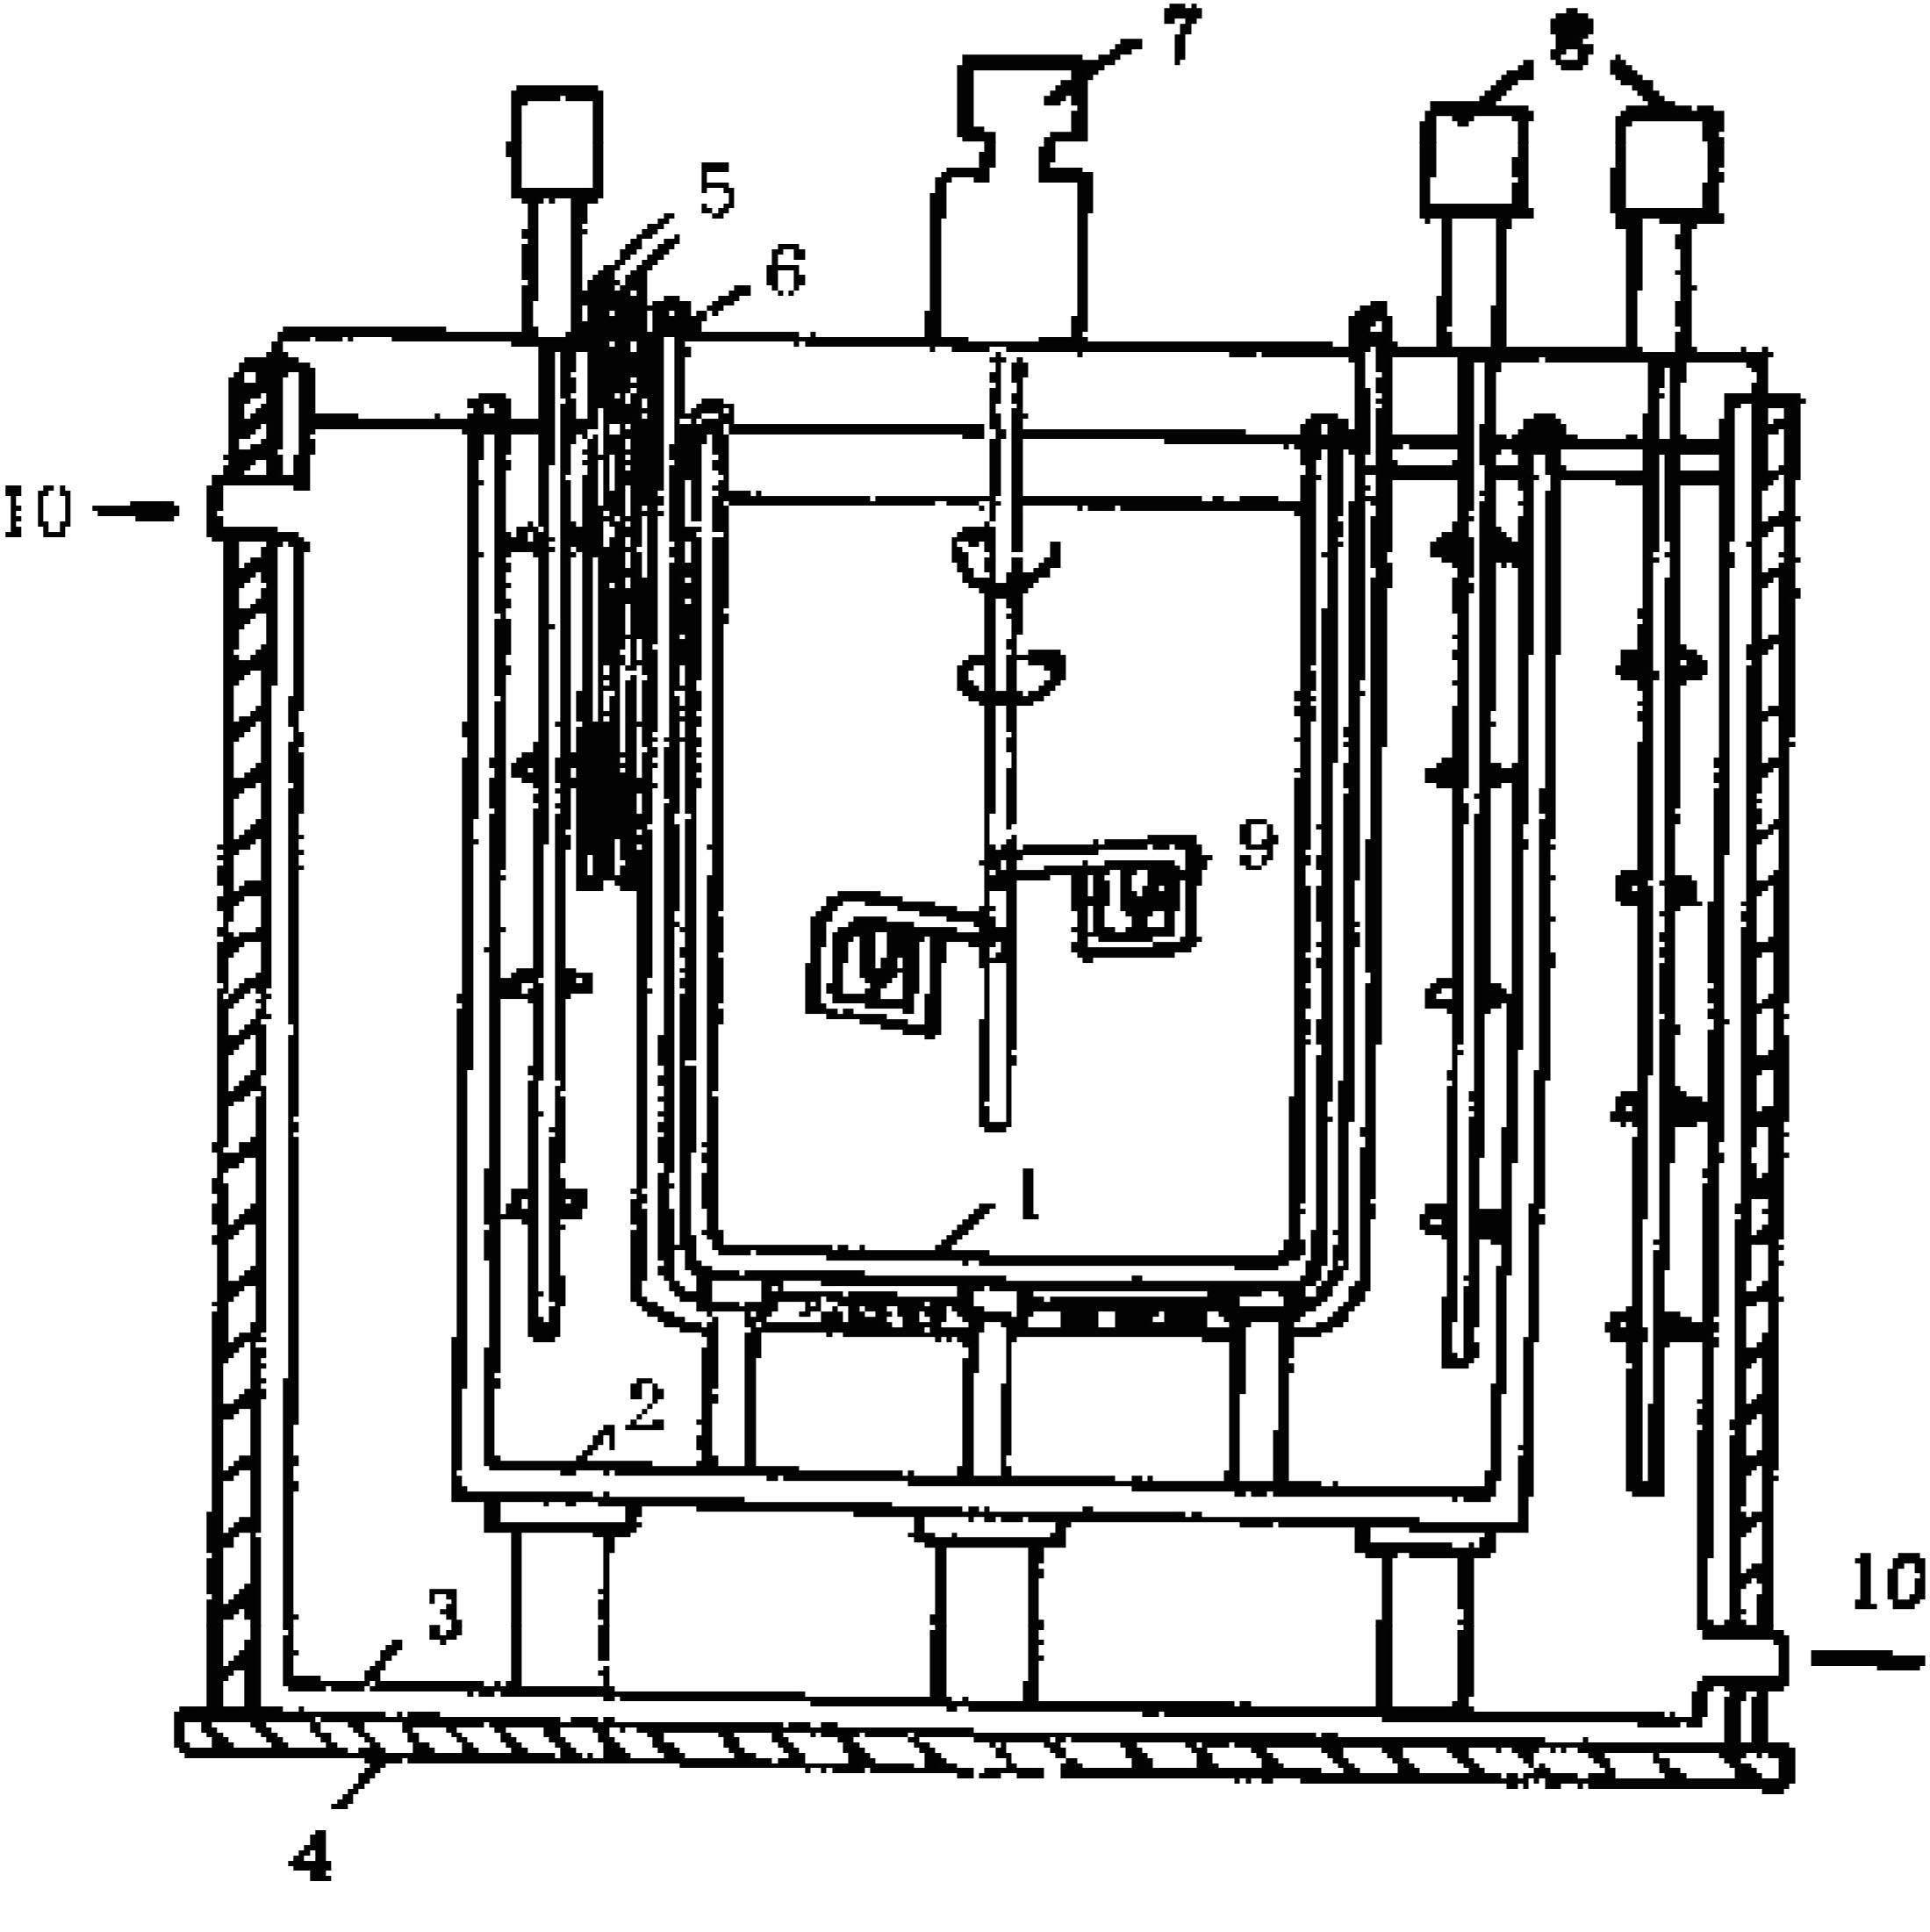
\includegraphics[width=0.45\textwidth]{fig/cp03/img3.20.jpg}
 \caption{双浴槽育晶装置。图中:}
 1为育晶器;2为内浴槽;3为外浴槽;4为保温层;5为感温元件;6为加热元件;7为转晶马达;8为搅拌马达(1500r/min);9为籽晶;10为外接冷却装置的进出口。
\end{figure}

为使溶液温度均匀,并使生长中的各个晶面在过饱和溶液中能得到均匀的溶质供应,要求晶体对溶液作相对运动。这种运动可采取多种形式,如晃动法(晶体固定不动,摇晃整个育晶器)、转晶法(晶体在溶液中作自转,公转或行星式转动)等,其中以晶体在溶液中自转或公转最为常用。为了克服这种方式所造成的的某些晶面迎液而动和使另一些晶面总是背向液流的缺点,转动需要定时换向,即用以下程序进行控制:正转---停转---反转---停转---正转。

降温法控制晶体生长的主要关键是掌握合适的降温速度。使溶液始终处于亚稳区内,并维持适宜的过饱和度,降温速度一般取决于以下述几个因素:
\begin{enumerate}[(1)]\itemsep -0.5ex
\item 晶体的最大透明生长速度(即在一定条件下不产生宏观缺陷的最大生长速度)。这一数值对不同晶体是有明显差别的(和亚稳区大小有关),例如对硝酸钠(NaNO$_3$)晶体为1mm/d,酒石酸钾钠(KNT)晶体则可达5mm/d以上。对同一晶体该数值还和晶体尺寸有关。
\item 溶解度的温度系数。溶解度的温度系数不但随不同物质而异,而且对同一种物质在不同的温度区间也一样。例如KDP的溶解度曲线在高温部分(50---70℃)温度系数较大,在低温部分(30℃以下)则较小。
\item 溶液的体积V(ml)和晶体生长表面积S(cm$^2$)之比,简称体面比。有些晶体(如KDP型晶体)在生长过程中,生长面积基本不变,而有些晶体(如KNT)在各个方向上都生长,S在生长过程中则在不断增加。
\end{enumerate}

总之,上述三个因素对于不同晶体是有明显差别的;对同一种晶体,这些因素在生长过程中也是在变化的。因此必须从实际出发,对不同的晶体在不同的阶段制定不同的降温程序。一般来说,在生长初期降温要慢,到了生长后期可稍快些。掌握规律后,可按程序实行自动降温。

必须指出,无宏观缺陷的晶体不一定是高质量的晶体(见3.4.3节)。培养用于光学目的高完整性的单晶,其生长速度应当控制的更小一些。

在控制降温过程中,最好能随时测定溶液的过饱和度(见3.1.4节)。同时,一些晶体生长现象[如生长涡流的强弱,晶面相对大小的变化,次要面的出现和消失,晶面花纹(见3.4.3节)等]往往是溶液过饱和度偏高或偏低以及晶体均匀性将遭破坏的“信号”。这些现象也可作为估计过饱和度、控制降温速度的参考信号。